\documentclass[letterpaper,11pt]{article}
\oddsidemargin -1.0cm \textwidth 17.5cm

\usepackage[utf8]{inputenc}
\usepackage[activeacute,spanish]{babel}
\usepackage{amsfonts,setspace}
\usepackage{amsmath}
\usepackage{amssymb, amsmath, amsthm}
\usepackage{comment}
\usepackage{amssymb}
\usepackage{dsfont}
\usepackage{anysize}
\usepackage{multicol}
\usepackage{enumerate}
\usepackage{graphicx}
\usepackage[left=1.5cm,top=2cm,right=1.5cm, bottom=1.7cm]{geometry}
\setlength\headheight{1.5em} 
\usepackage{fancyhdr}
\usepackage{multicol}
\usepackage{hyperref}
\usepackage{wrapfig}
\pagestyle{fancy}
\fancyhf{}
\renewcommand{\labelenumi}{\normalsize\bfseries P\arabic{enumi}.}
\renewcommand{\labelenumii}{\normalsize\bfseries (\alph{enumii})}
\renewcommand{\labelenumiii}{\normalsize\bfseries \roman{enumiii})}

\begin{document}
\fancyhead[L]{\itshape{Facultad de Ciencias F\'isicas y Matem\'aticas}}
\fancyhead[R]{\itshape{Universidad de Chile}}

\begin{minipage}{11.5cm}
    \begin{flushleft}
        \hspace*{-0.6cm}\textbf{FI1000-5 Introducción a la Física Clásica}\\
        \hspace*{-0.6cm}\textbf{Profesora:} Paulina Lira\\
        \hspace*{-0.6cm}\textbf{Auxiliares:} Alejandro Silva, Juan Cristóbal Castro\\
    \end{flushleft}
\end{minipage}

\begin{picture}(2,3)
    \put(405,-5){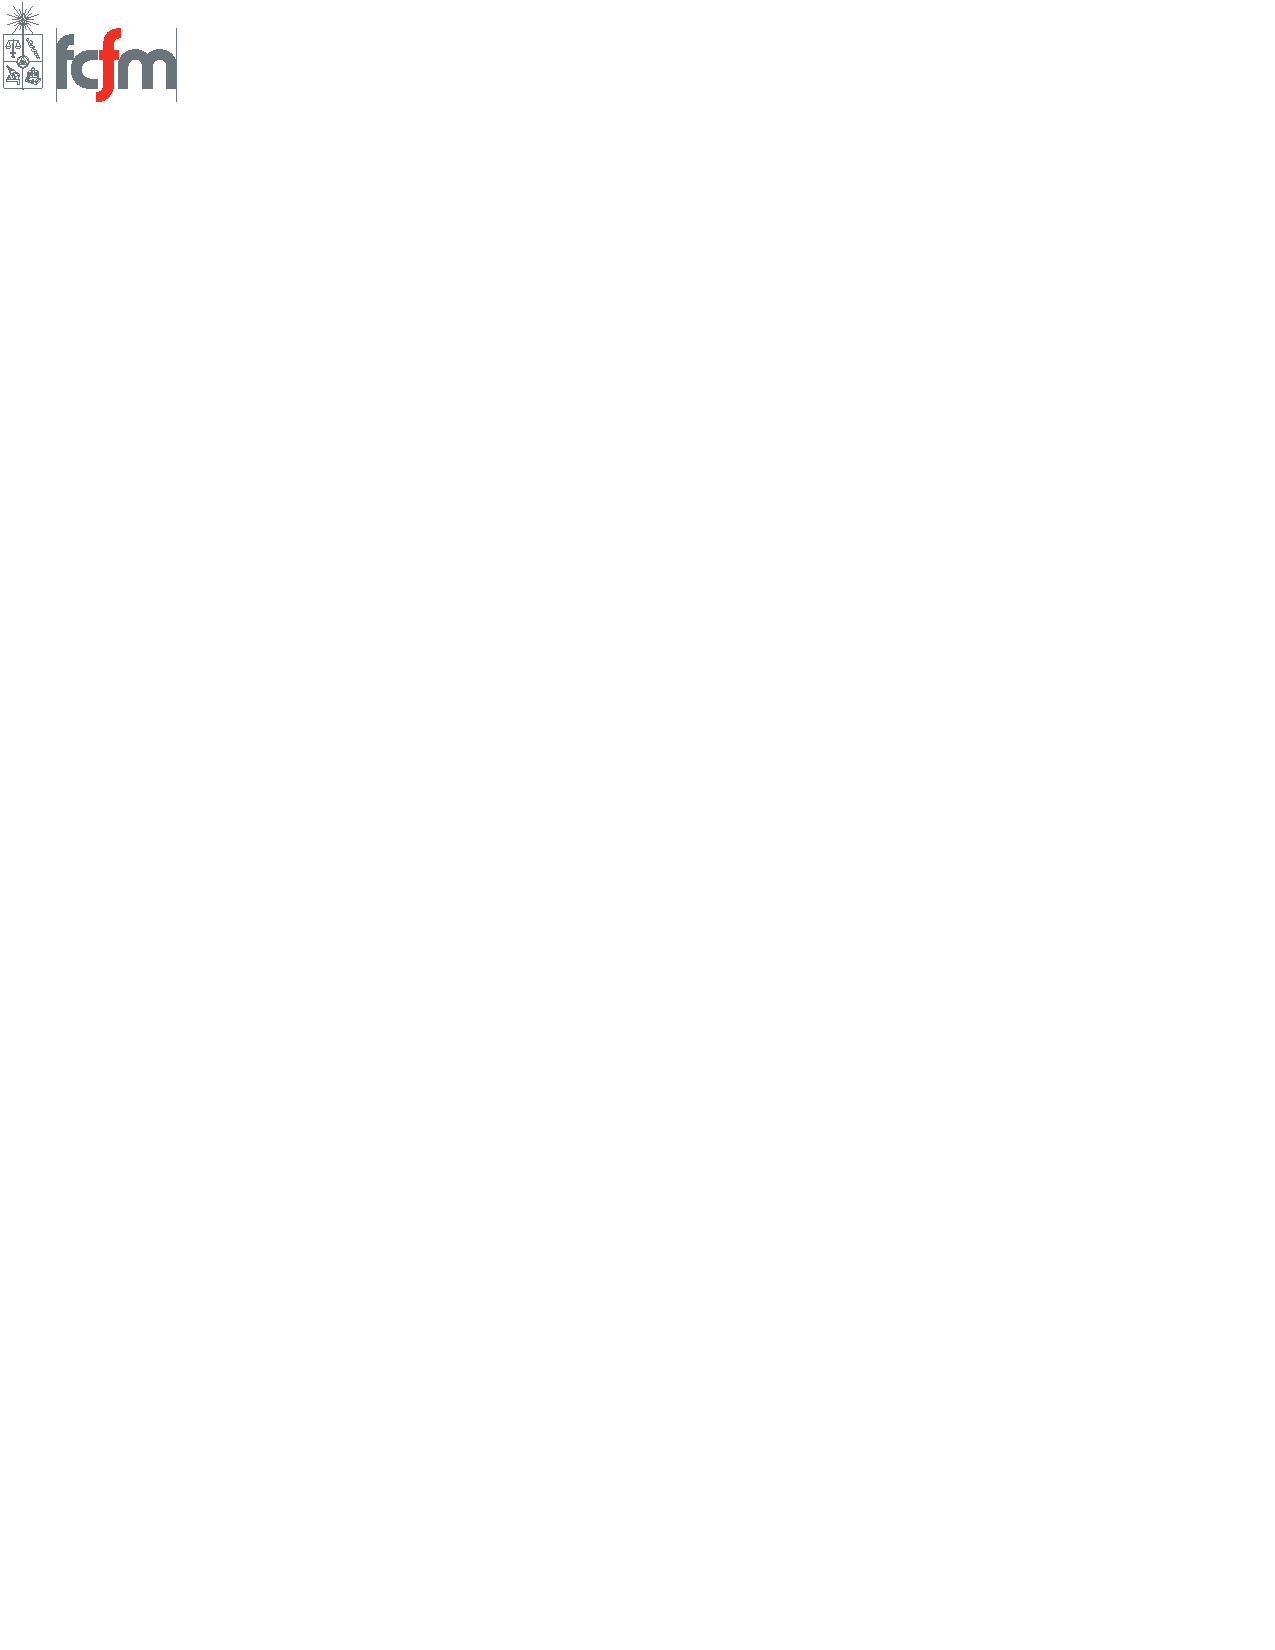
\includegraphics[scale=1.25]{2020-1/Imágenes/logo/fcfm2.pdf}}
\end{picture}

\begin{center}
	\LARGE \bf Auxiliar \#1: Intro a la Cinemática  \\
\end{center}

\vspace{-1cm}
\begin{enumerate}\setlength{\itemsep}{0.4cm}

\rfoot[]{pág. \thepage}\\
\\
\item[]
\item En el gráfico adjunto se representa la velocidad en función del tiempo para dos móviles, A y B, desplazándose a lo largo de un mismo trayecto rectilíneo. Se sabe además que cuando A alcanza la misma velocidad que B, ambos móviles se encuentran uno junto al otro. Determine la ubicación inicial de B si la posición inicial de A es A(t = 0) = 25 m.
    \begin{figure}[h!]
        \centering
        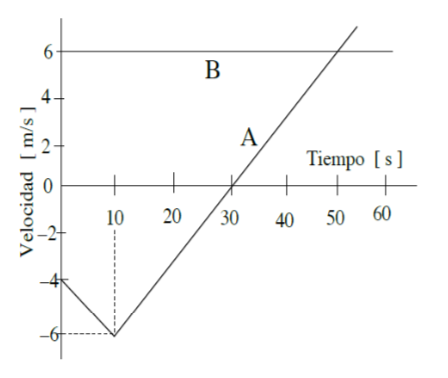
\includegraphics[scale=0.3]{2020-1/Imágenes/aux2/plot.png}
    \end{figure}
\item Se tiene el siguiente gráfico que esquematiza el movimiento de una partícula:
    \begin{figure}[h!]
        \centering
        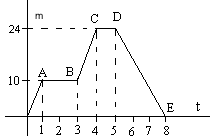
\includegraphics[scale=0.6]{2020-1/Imágenes/aux2/grafo.png}
    \end{figure}

\begin{enumerate}
    \item Calcule la velocidad media entre los puntos:
        \begin{enumerate}
            \item A-B
            \item A-C
            \item D-E
        \end{enumerate}
    \item Calcule la velocidad instantánea a los:
        \begin{enumerate}
            \item 3,5 seg.
            \item 2 seg.
            \item 6,8 seg.
        \end{enumerate}
\end{enumerate}
 \item Dos partículas A y B se encuentran separadas sobre un trayecto rectilíneo, estas se encuentran en $x_a$ y $x_b$, con $x_a<x_b$. En t=0 comienzan a moverse una hacia la otra con velocidades $v_a$ y $v_b$ respectivamente. Determine el tiempo y la posición de choque. 

\item Una bola se deja caer desde una altura h. Al mismo tiempo, un carro que se encuentra a una distancia horizontal $x_c$ comienza a moverse con velocidad $v_c$ hacia la bola. 
Determine la altura h tal que la bolita caiga dentro del carro. 

\end{enumerate}
\end{document}